\documentclass{beamer}

\mode<presentation>
{
  \usetheme{Berkeley}
  \setbeamercovered{transparent}
}

\usepackage[absolute,overlay]{textpos}
\usepackage{graphicx}
\usepackage{color}
\usepackage{epsfig}
\usepackage[english]{babel}
\usepackage{listings}
\usepackage{graphics}
\usepackage{subfigure}

\setlength{\TPHorizModule}{1cm}
\setlength{\TPVertModule}{\TPHorizModule}
\textblockorigin{1cm}{1cm} % start everything near the top-left corner
\setlength{\parindent}{0pt}

\title{Data Dissemination: from Academia to Industry}

\author{\textbf{Jo{\~a}o Leit{\~a}o}\\NOVA-LINCS \& NOVA University of Lisbon
\\\textbf{Jordan West}\\BASHO Inc.
}
\date{RICON\\Las Vegas\\October 2014}

\begin{document}
%\definecolor{links}{rgb}{0.2116,0.0104,0.7716}
%\definecolor{highlight}{rgb}{1,1,0.1}


\frame{

\titlepage

}

\section{Motivation}

\frame
{
	\frametitle{Outline}
{
\small
	\tableofcontents[hideallsubsections]
}
}

\frame
{
	\frametitle{Outline}
{
\small
	\tableofcontents[currentsection,hideallsubsections]
}
}

\frame{

\frametitle{Motivation}
\framesubtitle{Data Dissemination}

\begin{block}{Classical Distributed Systems Challenge}
How to disseminate information across a large number of participants?
\end{block}

\pause

\begin{itemize}
\item Some intuitive requirements:
\begin{itemize}
	\item Reliable.
	\item Efficient.
	\item Scalable.
\end{itemize}
\end{itemize}

}

\frame{

\frametitle{Motivation}
\framesubtitle{Data Dissemination}

\begin{block}{Applications}
\begin{itemize}
	\item Notification systems.
	\item Streaming multimedia content.
	\item \emph{Cluster Management}
\end{itemize}
\end{block}

\pause

\begin{block}{In practice...}
When I started to think about this problem, I was mostly focused on peer-to-peer systems.
\end{block}}

\section{The Academic View: Data Dissemination}

\frame
{
	\frametitle{Outline}
{
\small
	\tableofcontents[currentsection,hideallsubsections]
}
}

\frame
{
	\frametitle{Outline}
{
\small
	\tableofcontents[currentsection,hideallsubsections]
}
}

\subsection{Design Alternatives: One to All}

\frame{
\frametitle{The Academic View: Data Dissemination}
\framesubtitle{Design Alternatives: One to All}

\begin{figure}[h]
  \begin{center}
  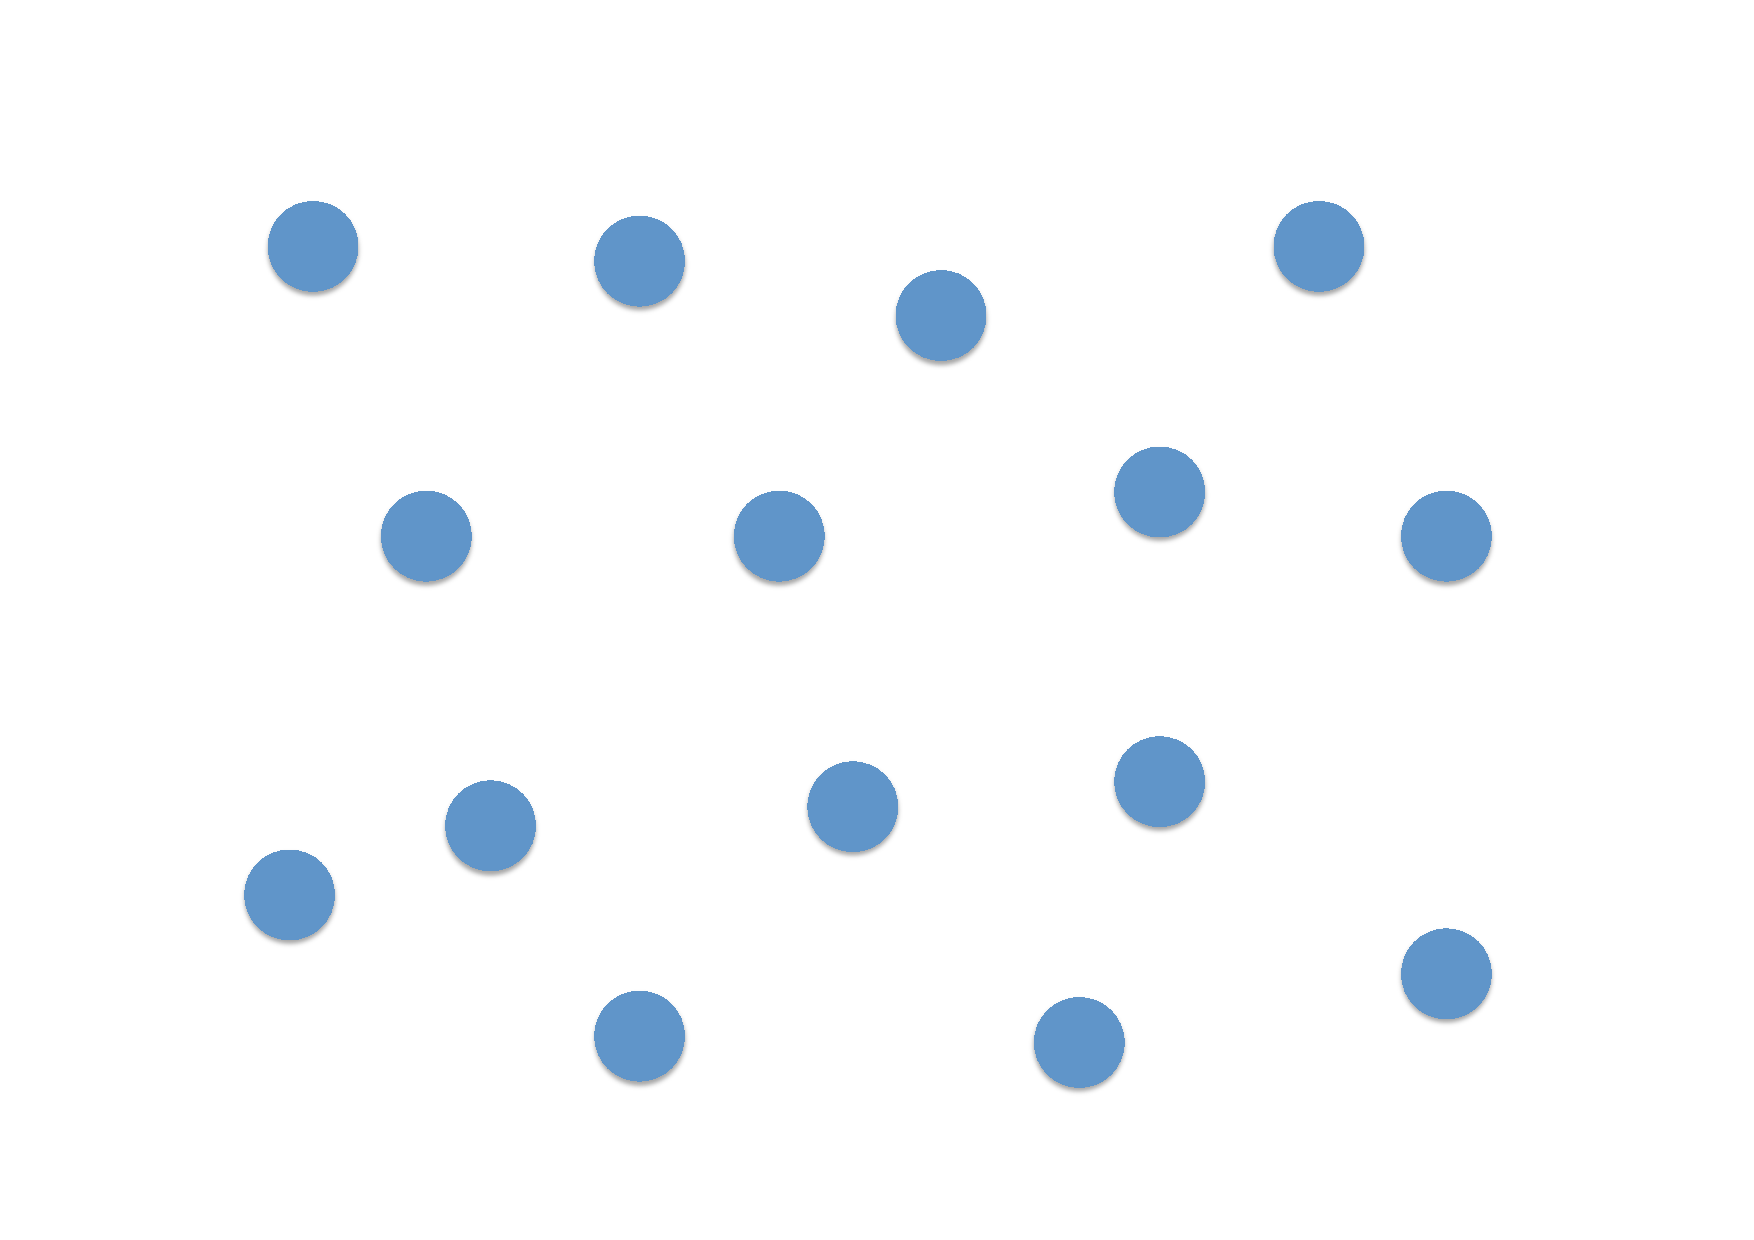
\includegraphics[width=1\textwidth]{pics/one2all1}
  \end{center}
\end{figure}

}

\frame{
\frametitle{The Academic View: Data Dissemination}
\framesubtitle{Design Alternatives: One to All}

\begin{figure}[h]
  \begin{center}
  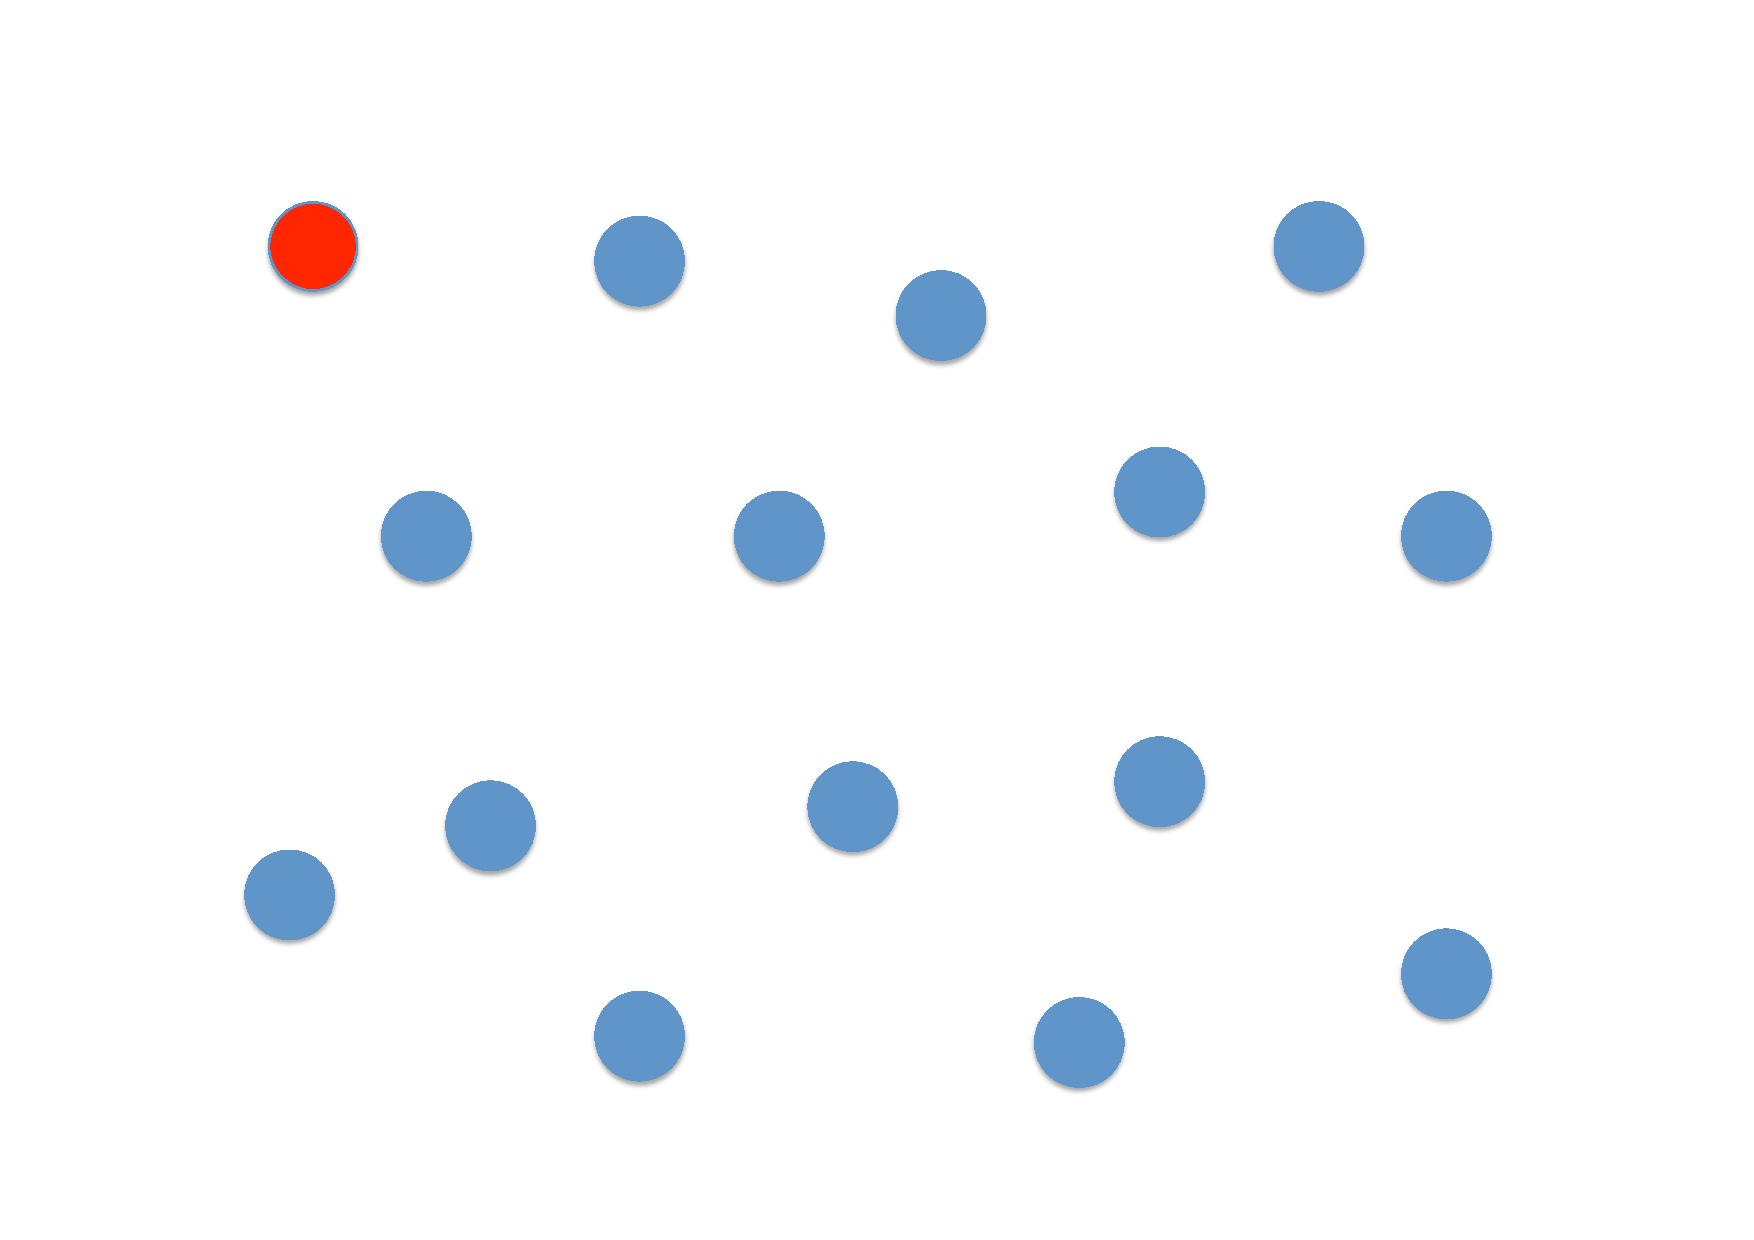
\includegraphics[width=1\textwidth]{pics/one2all2}
  \end{center}
\end{figure}

}

\frame{
\frametitle{The Academic View: Data Dissemination}
\framesubtitle{Design Alternatives: One to All}

\begin{figure}[h]
  \begin{center}
  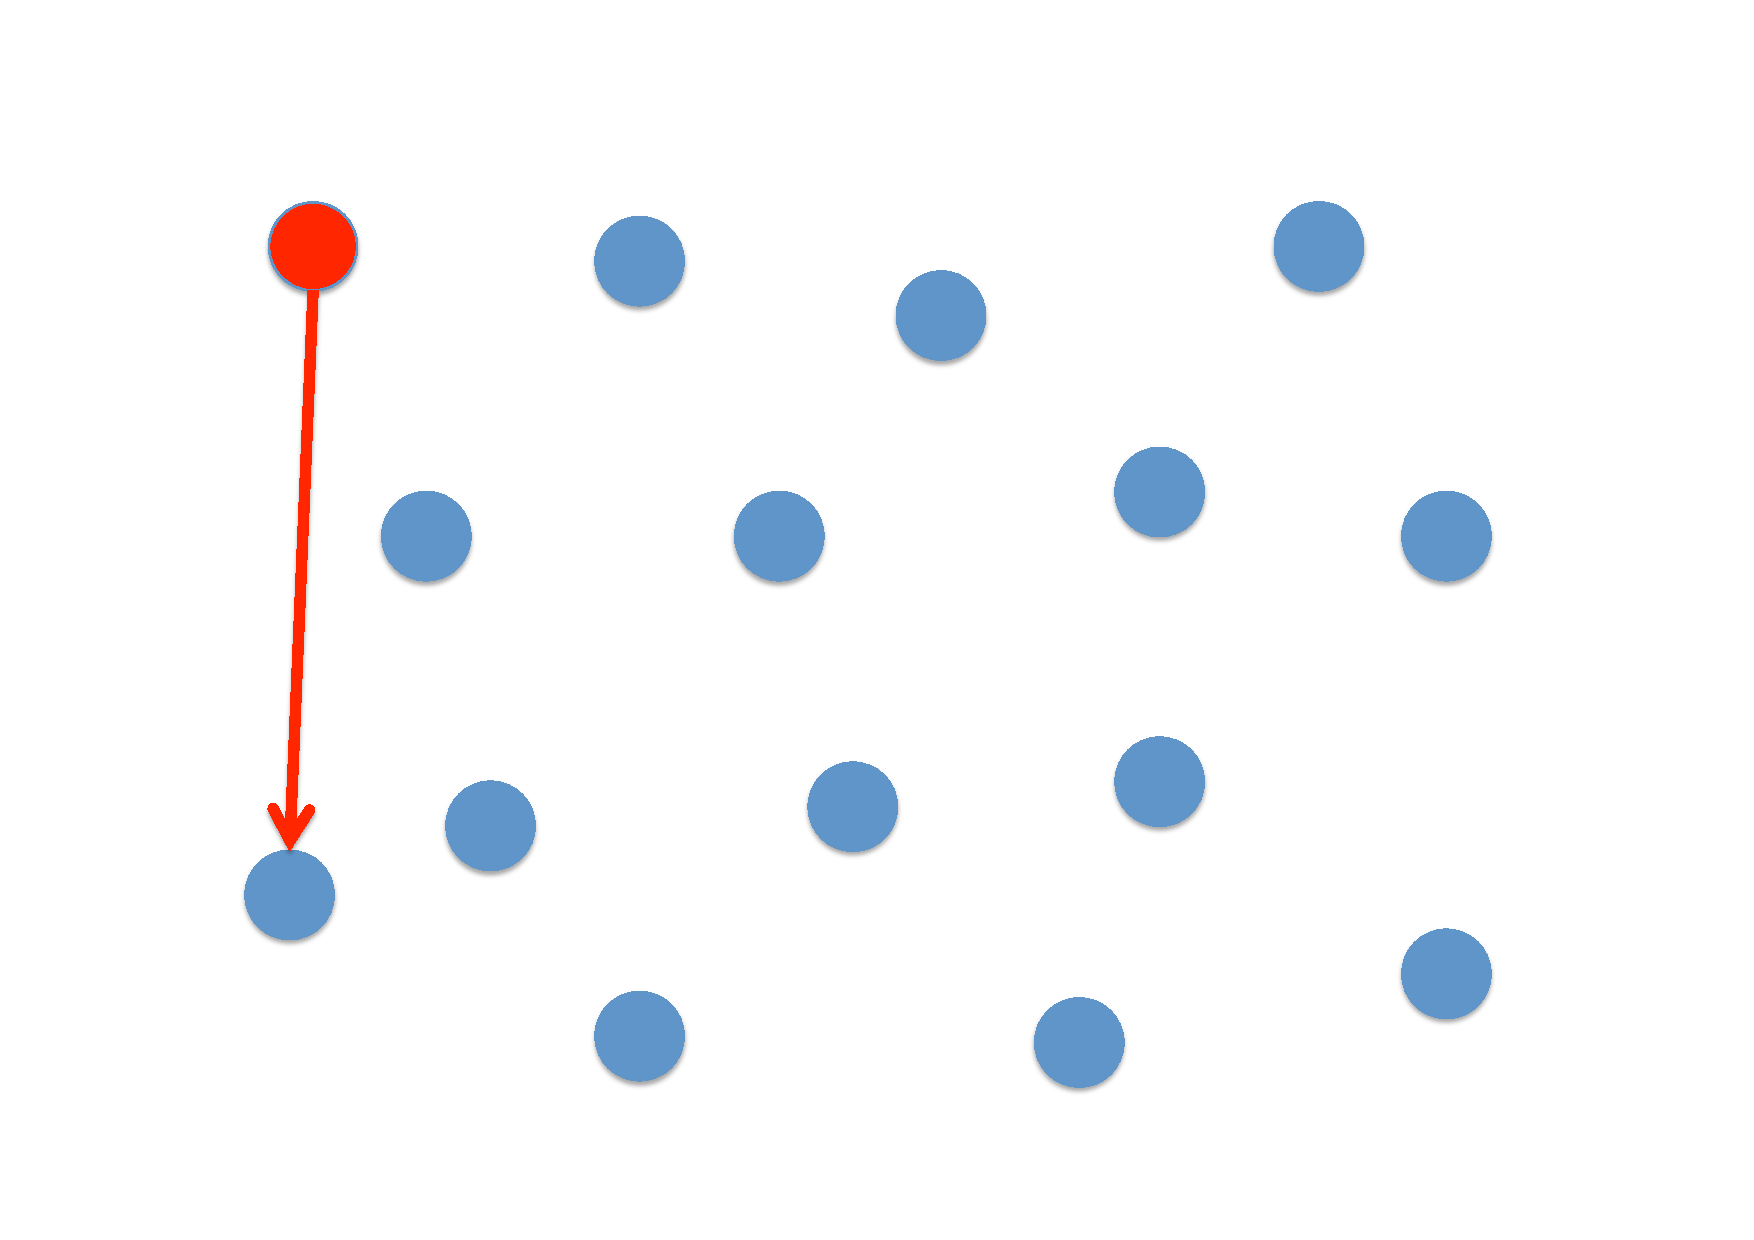
\includegraphics[width=1\textwidth]{pics/one2all3}
  \end{center}
\end{figure}

}

\frame{
\frametitle{The Academic View: Data Dissemination}
\framesubtitle{Design Alternatives: One to All}

\begin{figure}[h]
  \begin{center}
  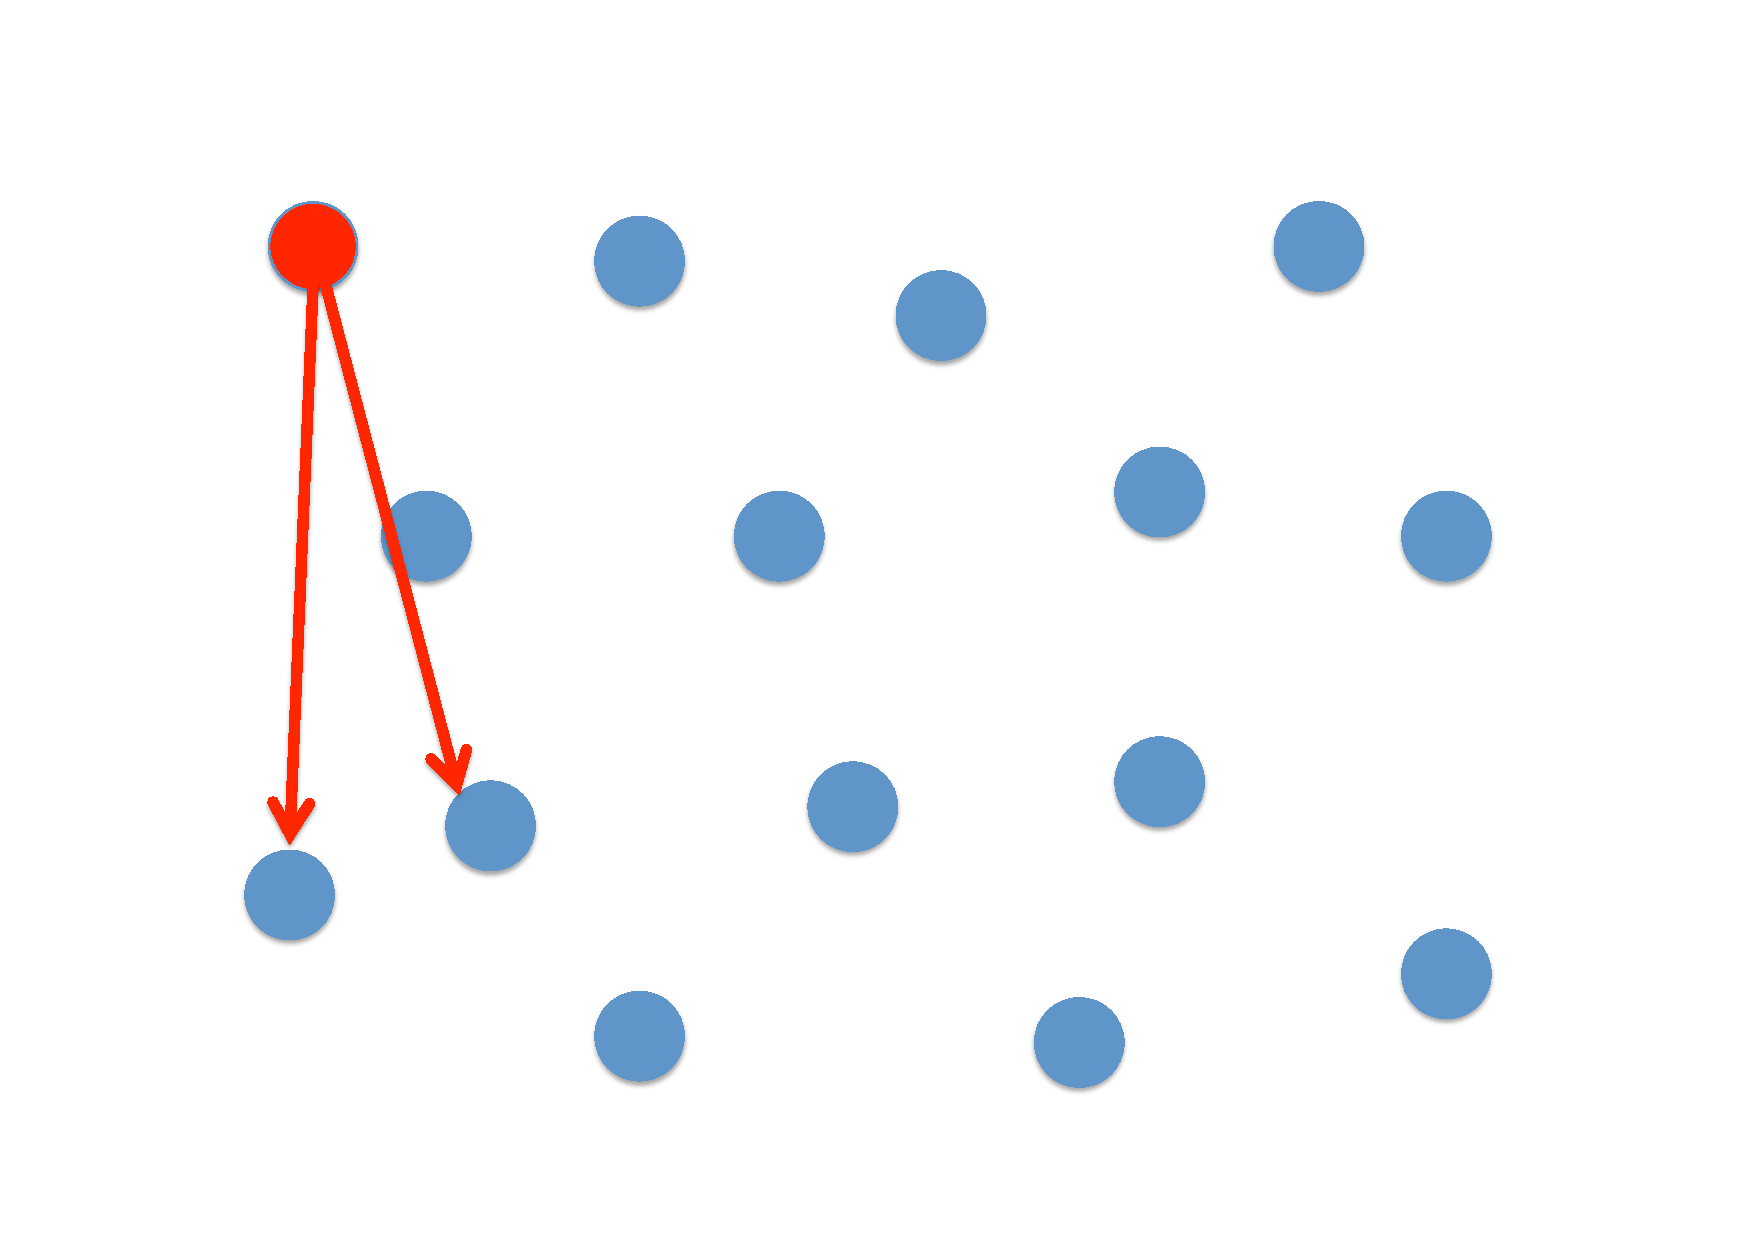
\includegraphics[width=1\textwidth]{pics/one2all4}
  \end{center}
\end{figure}

}

\frame{
\frametitle{The Academic View: Data Dissemination}
\framesubtitle{Design Alternatives: One to All}

\begin{figure}[h]
  \begin{center}
  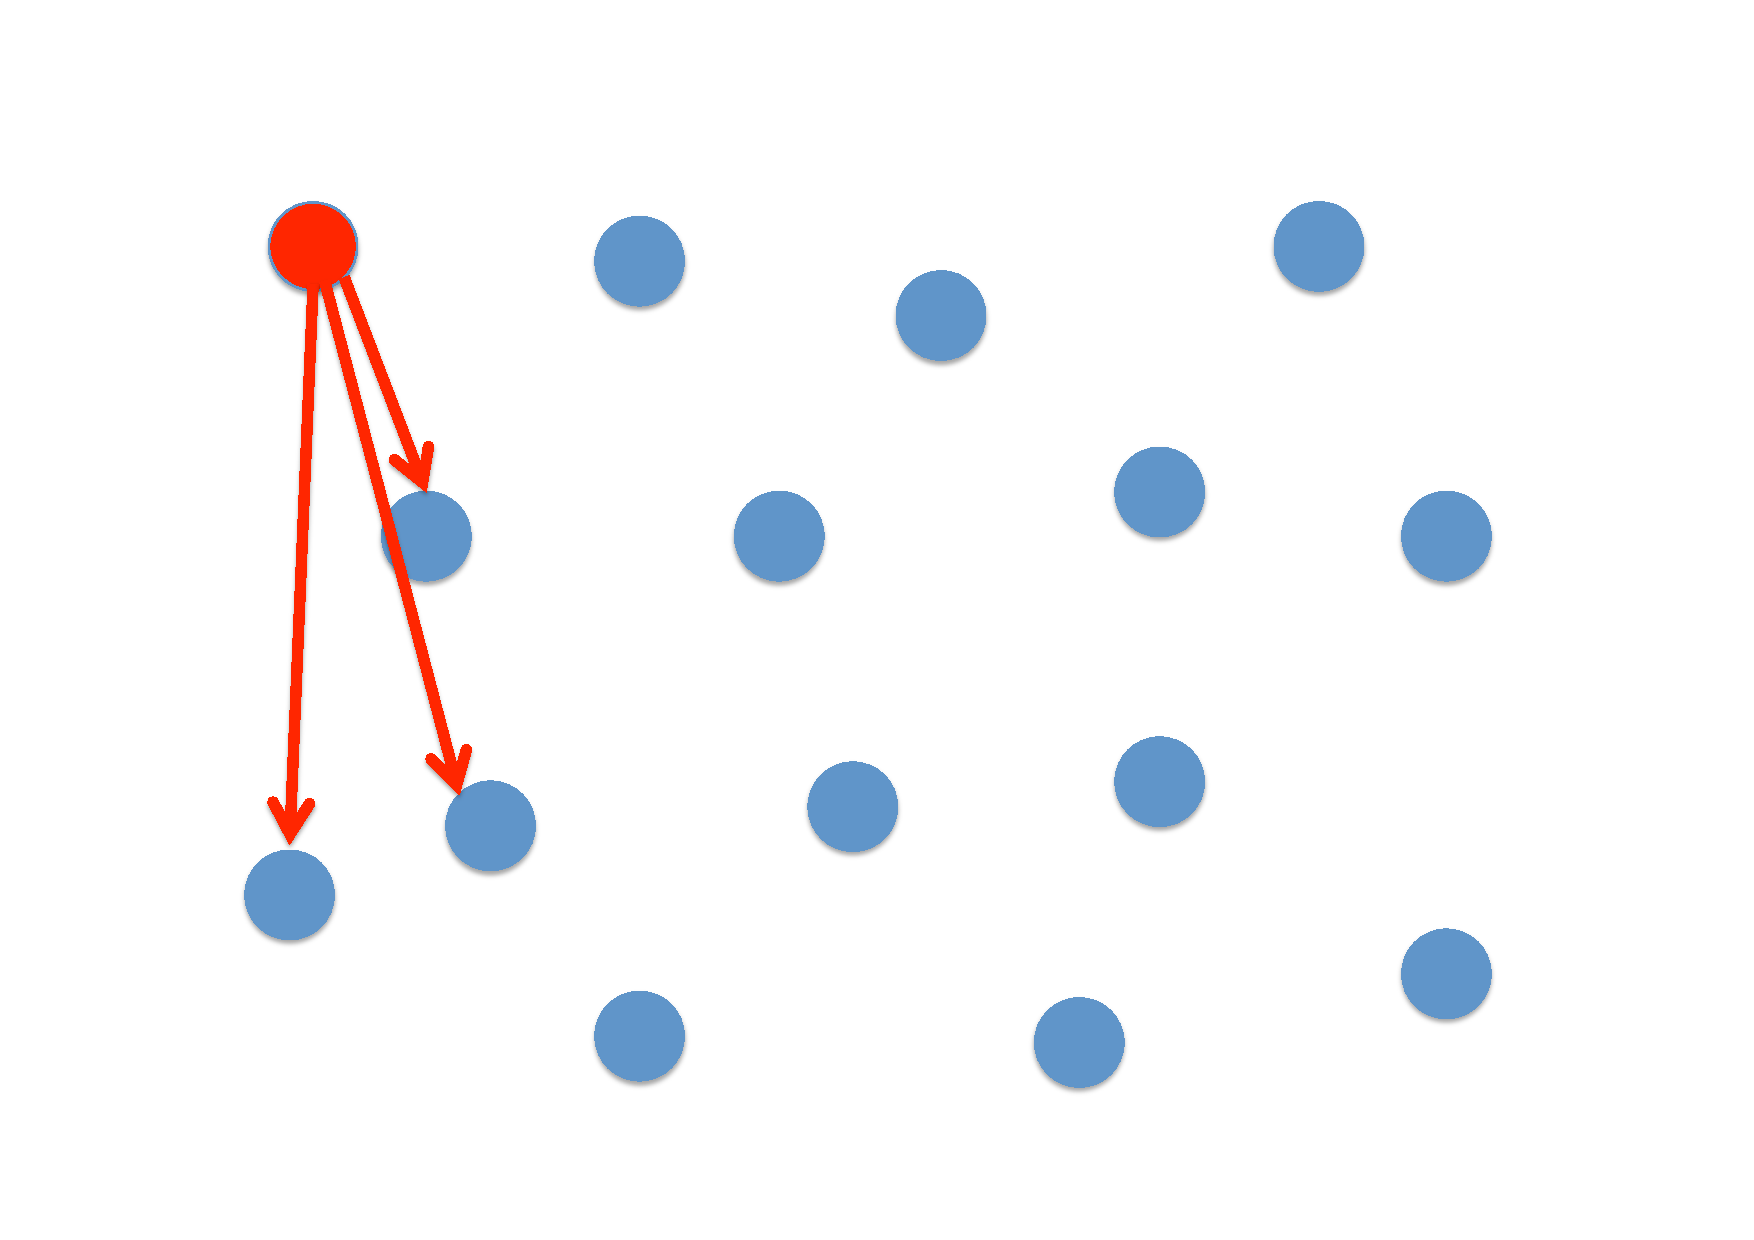
\includegraphics[width=1\textwidth]{pics/one2all5}
  \end{center}
\end{figure}

}

\frame{
\frametitle{The Academic View: Data Dissemination}
\framesubtitle{Design Alternatives: One to All}

\begin{figure}[h]
  \begin{center}
  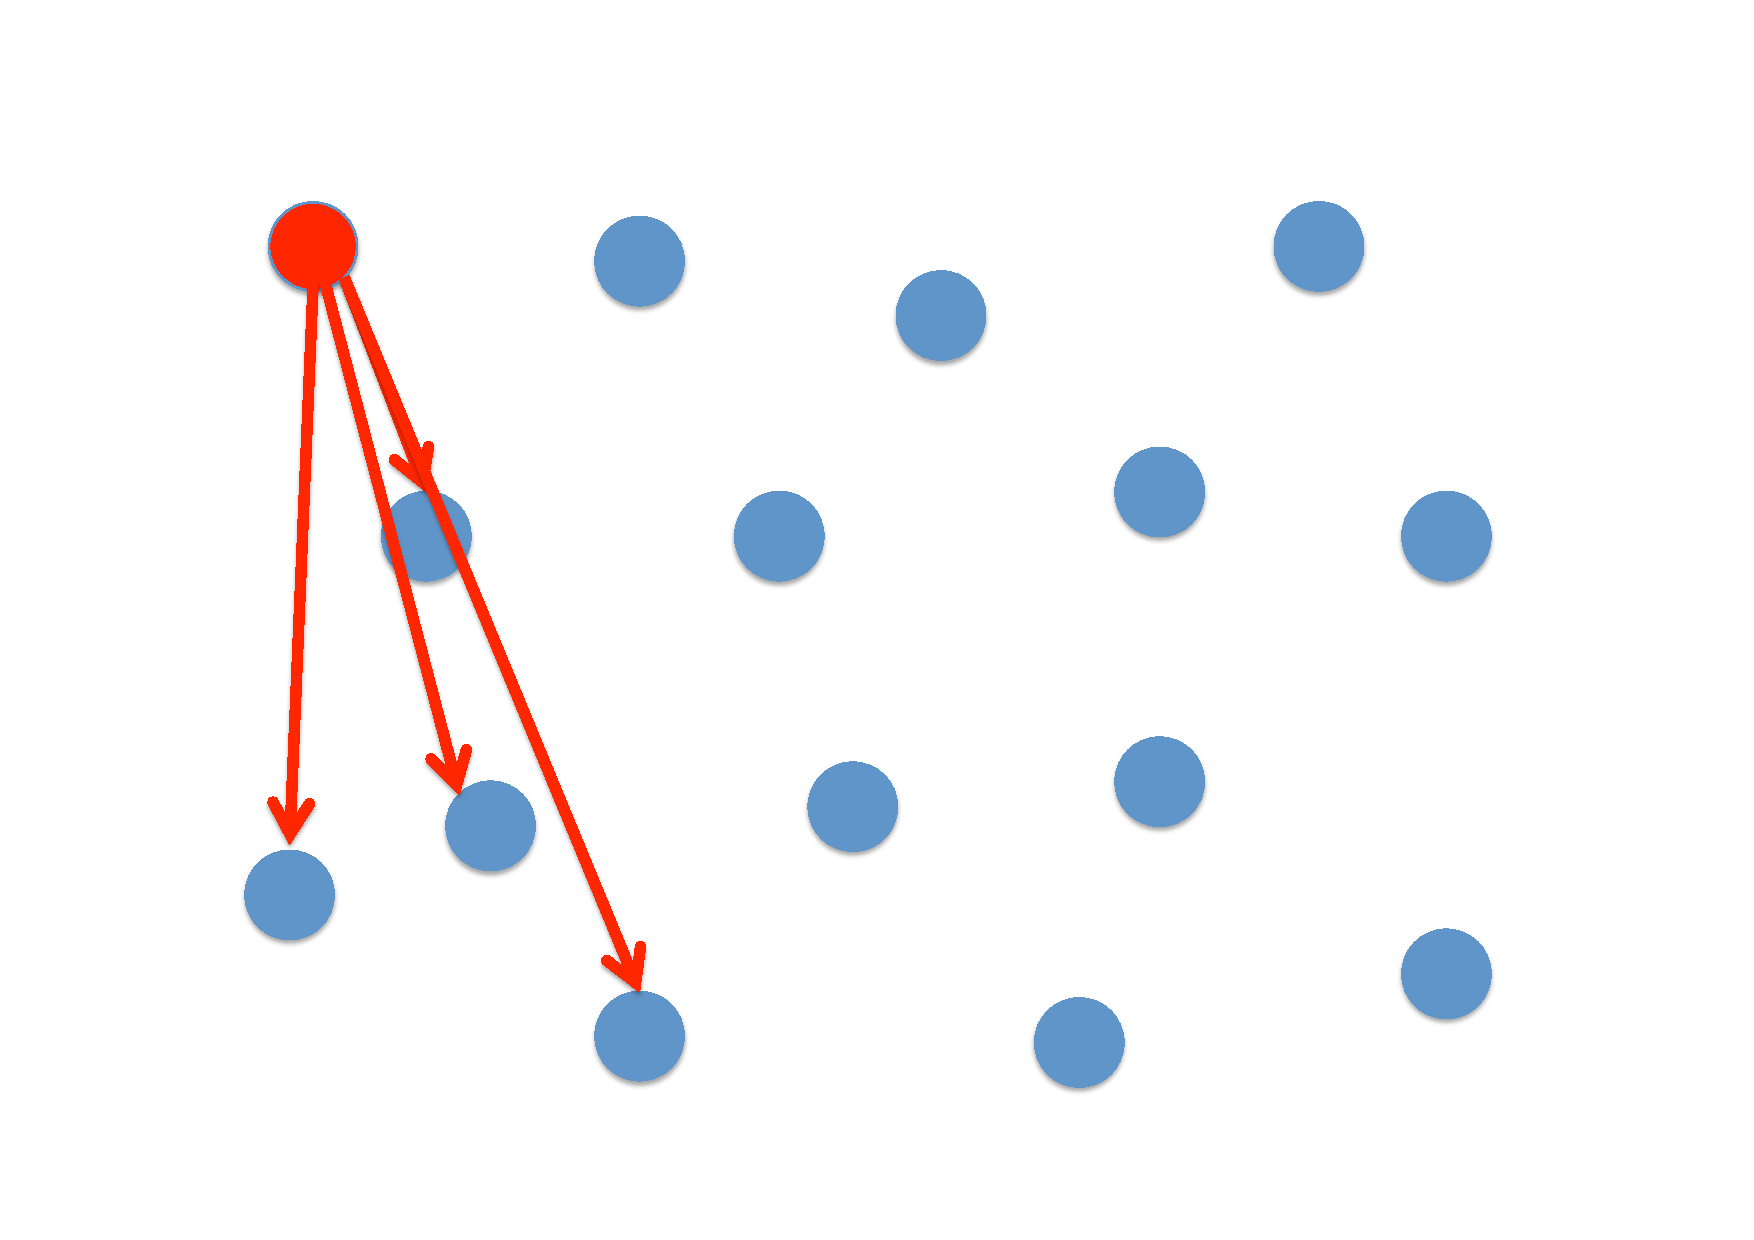
\includegraphics[width=1\textwidth]{pics/one2all6}
  \end{center}
\end{figure}

}

\frame{
\frametitle{The Academic View: Data Dissemination}
\framesubtitle{Design Alternatives: One to All}

\begin{figure}[h]
  \begin{center}
  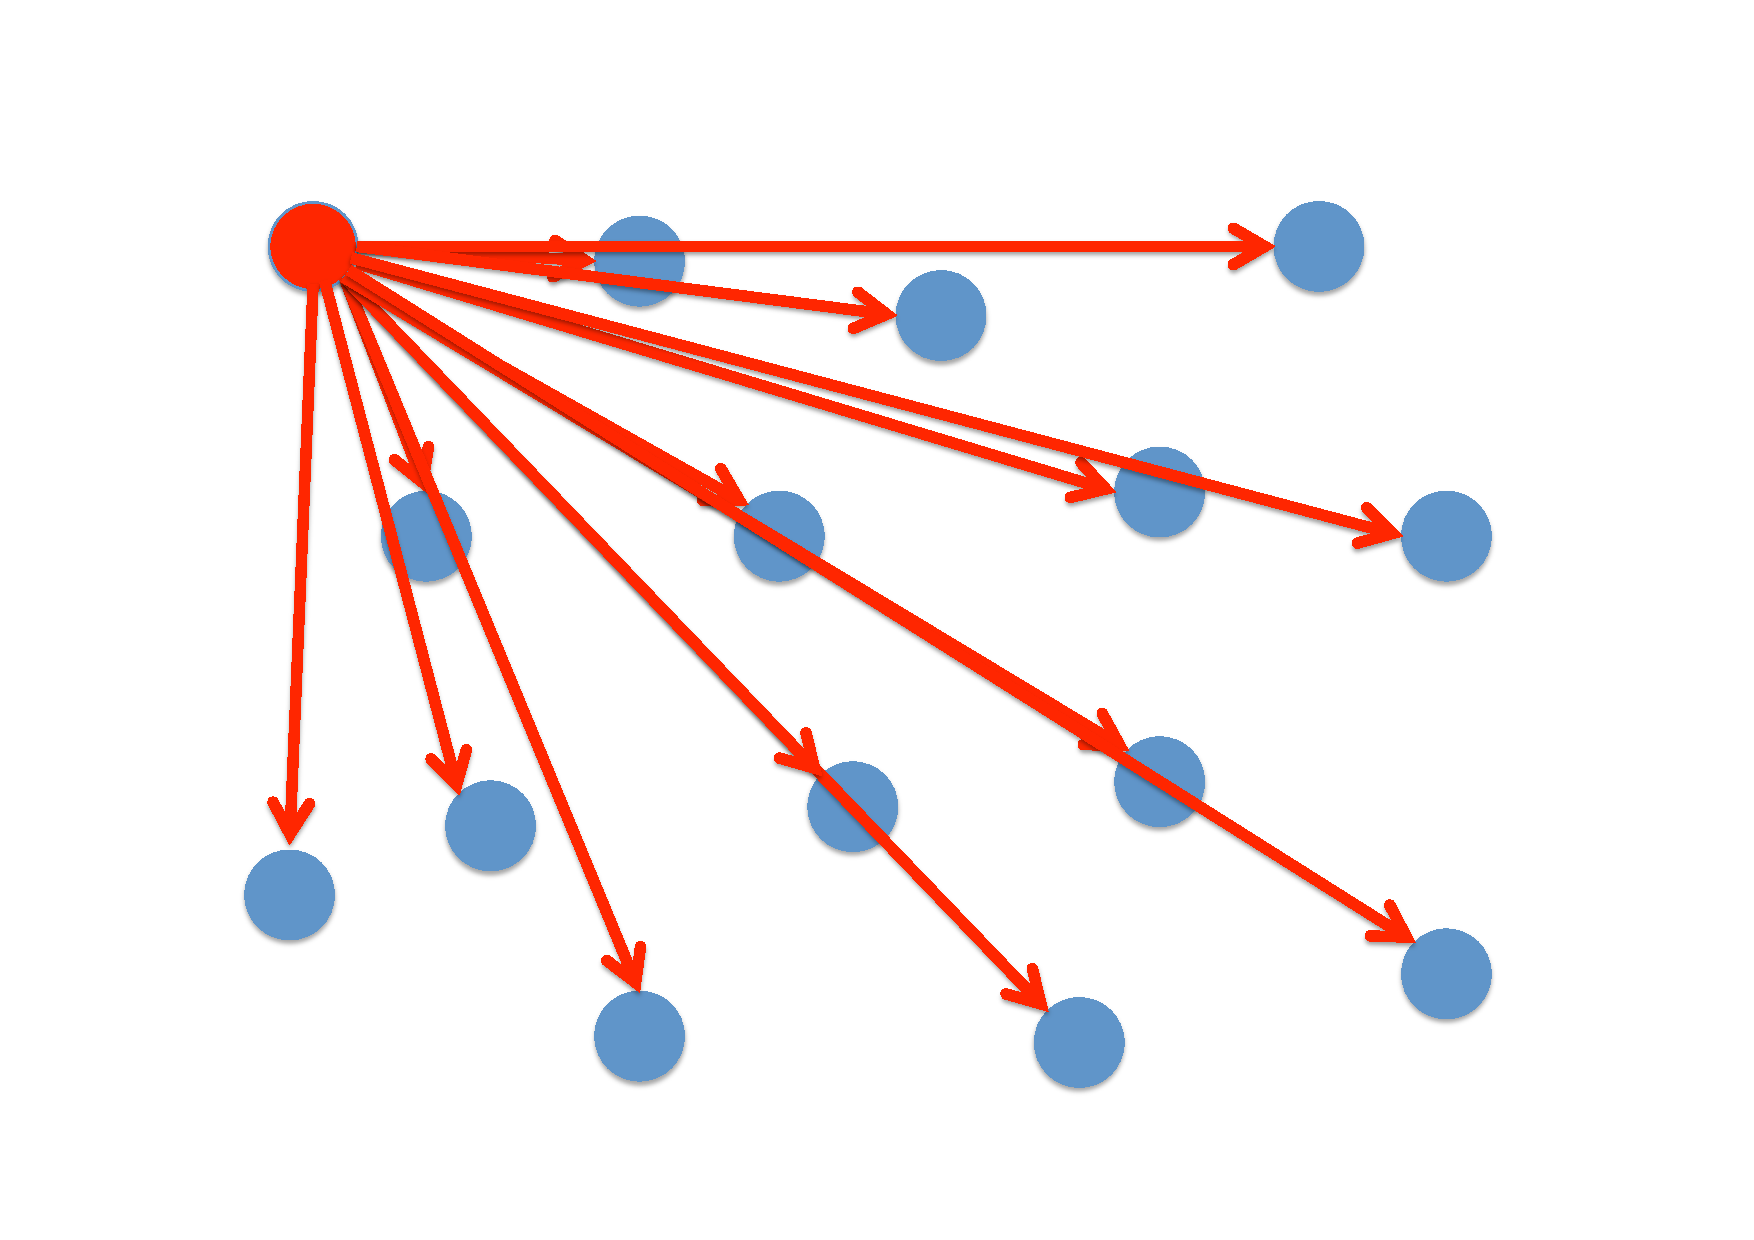
\includegraphics[width=1\textwidth]{pics/one2all7}
  \end{center}
\end{figure}

}

\frame{
\frametitle{The Academic View: Data Dissemination}
\framesubtitle{Design Alternatives: One to All}

\begin{block}{One to All}
	\begin{itemize}
		\item Positive Aspects:
		\begin{itemize}
			\item Straight forward.
			\item No redundancy (i.e, each node receives each message a single time).
		\end{itemize}
	\end{itemize}
	
	\pause
	
	\begin{itemize}
		\item Negative Aspects:
		\begin{itemize}
			\item Requires each node to know the full membership.
			\item Not Scalable (no load distribution).
			\pause
			\item Not Resilient to Faults.
		\end{itemize}
	\end{itemize}
\end{block}
}

\frame{
\frametitle{The Academic View: Data Dissemination}
\framesubtitle{Design Alternatives: One to All}

\begin{figure}[h]
  \begin{center}
  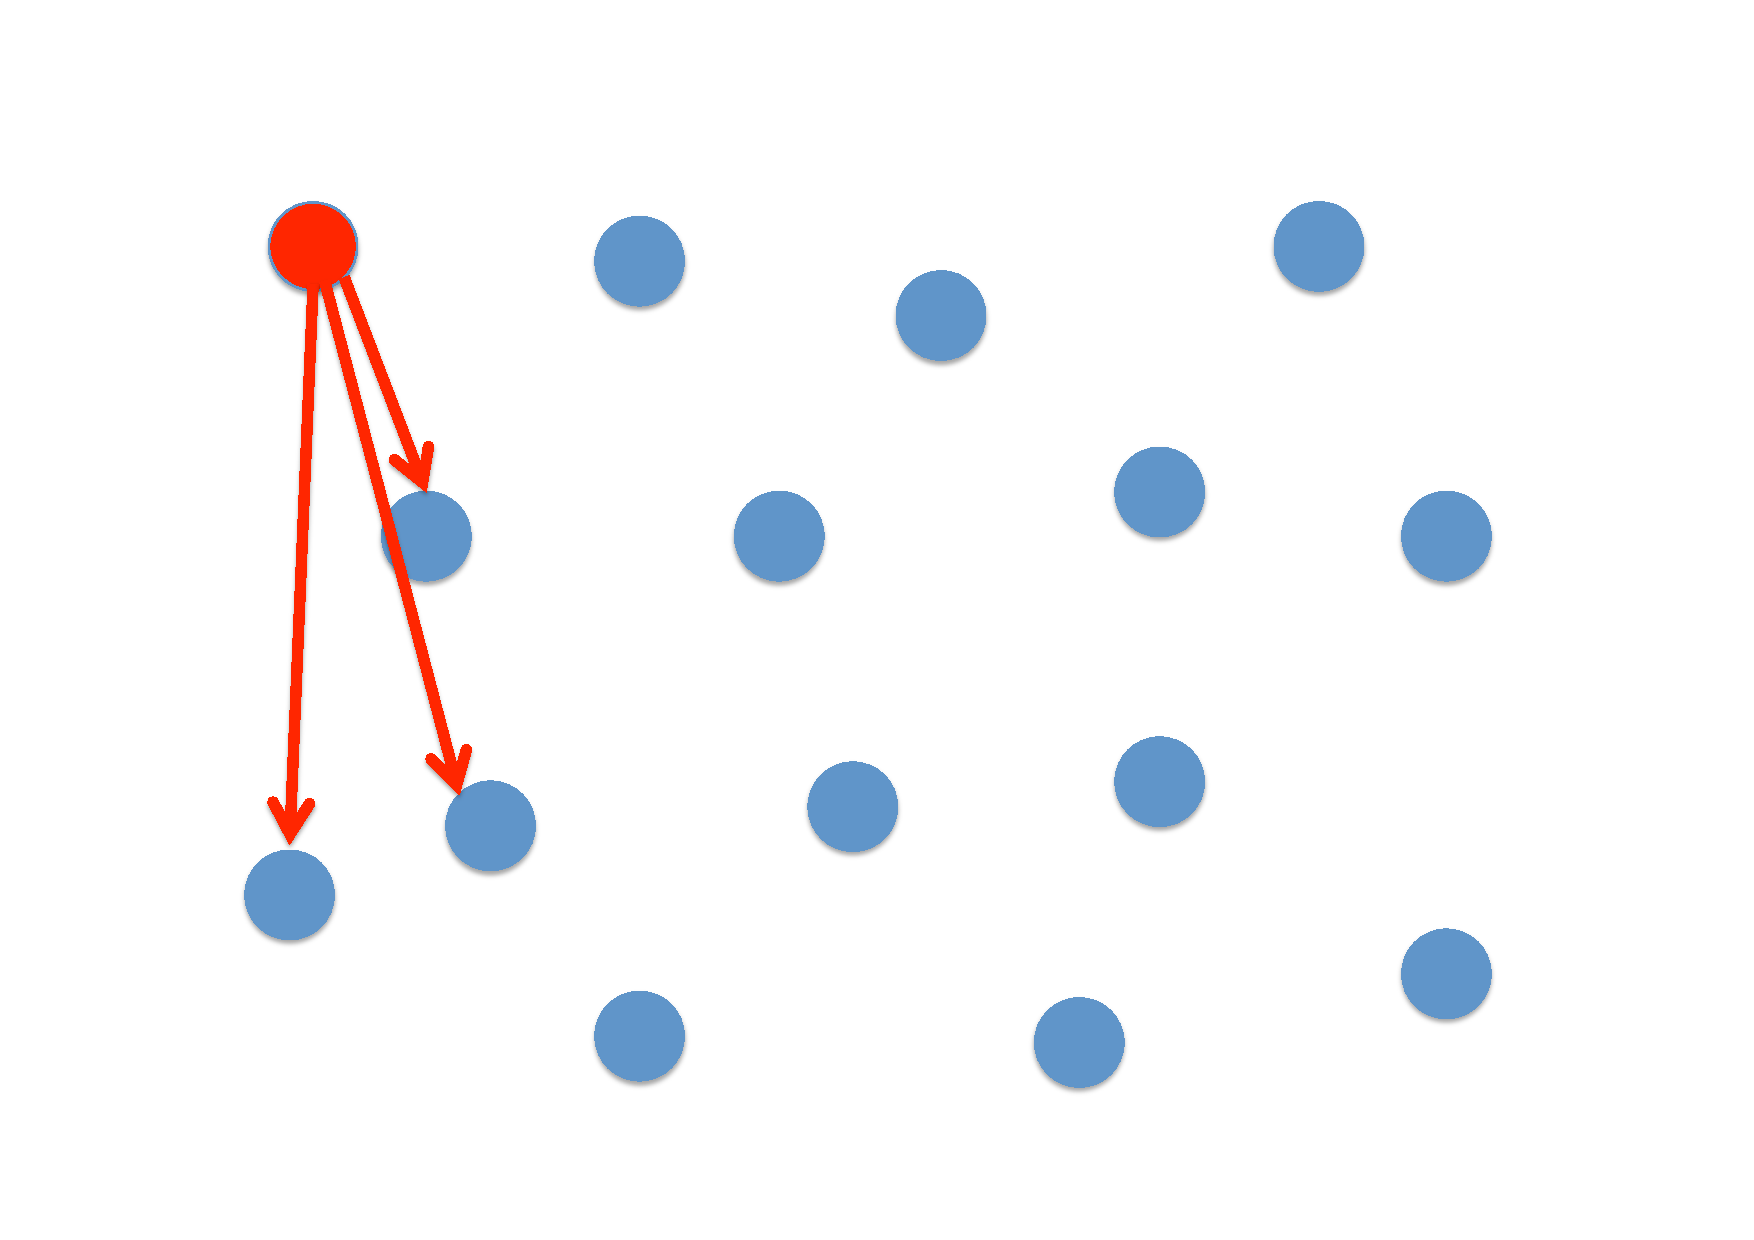
\includegraphics[width=1\textwidth]{pics/fault1}
  \end{center}
\end{figure}

}

\frame{
\frametitle{The Academic View: Data Dissemination}
\framesubtitle{Design Alternatives: One to All}

\begin{figure}[h]
  \begin{center}
  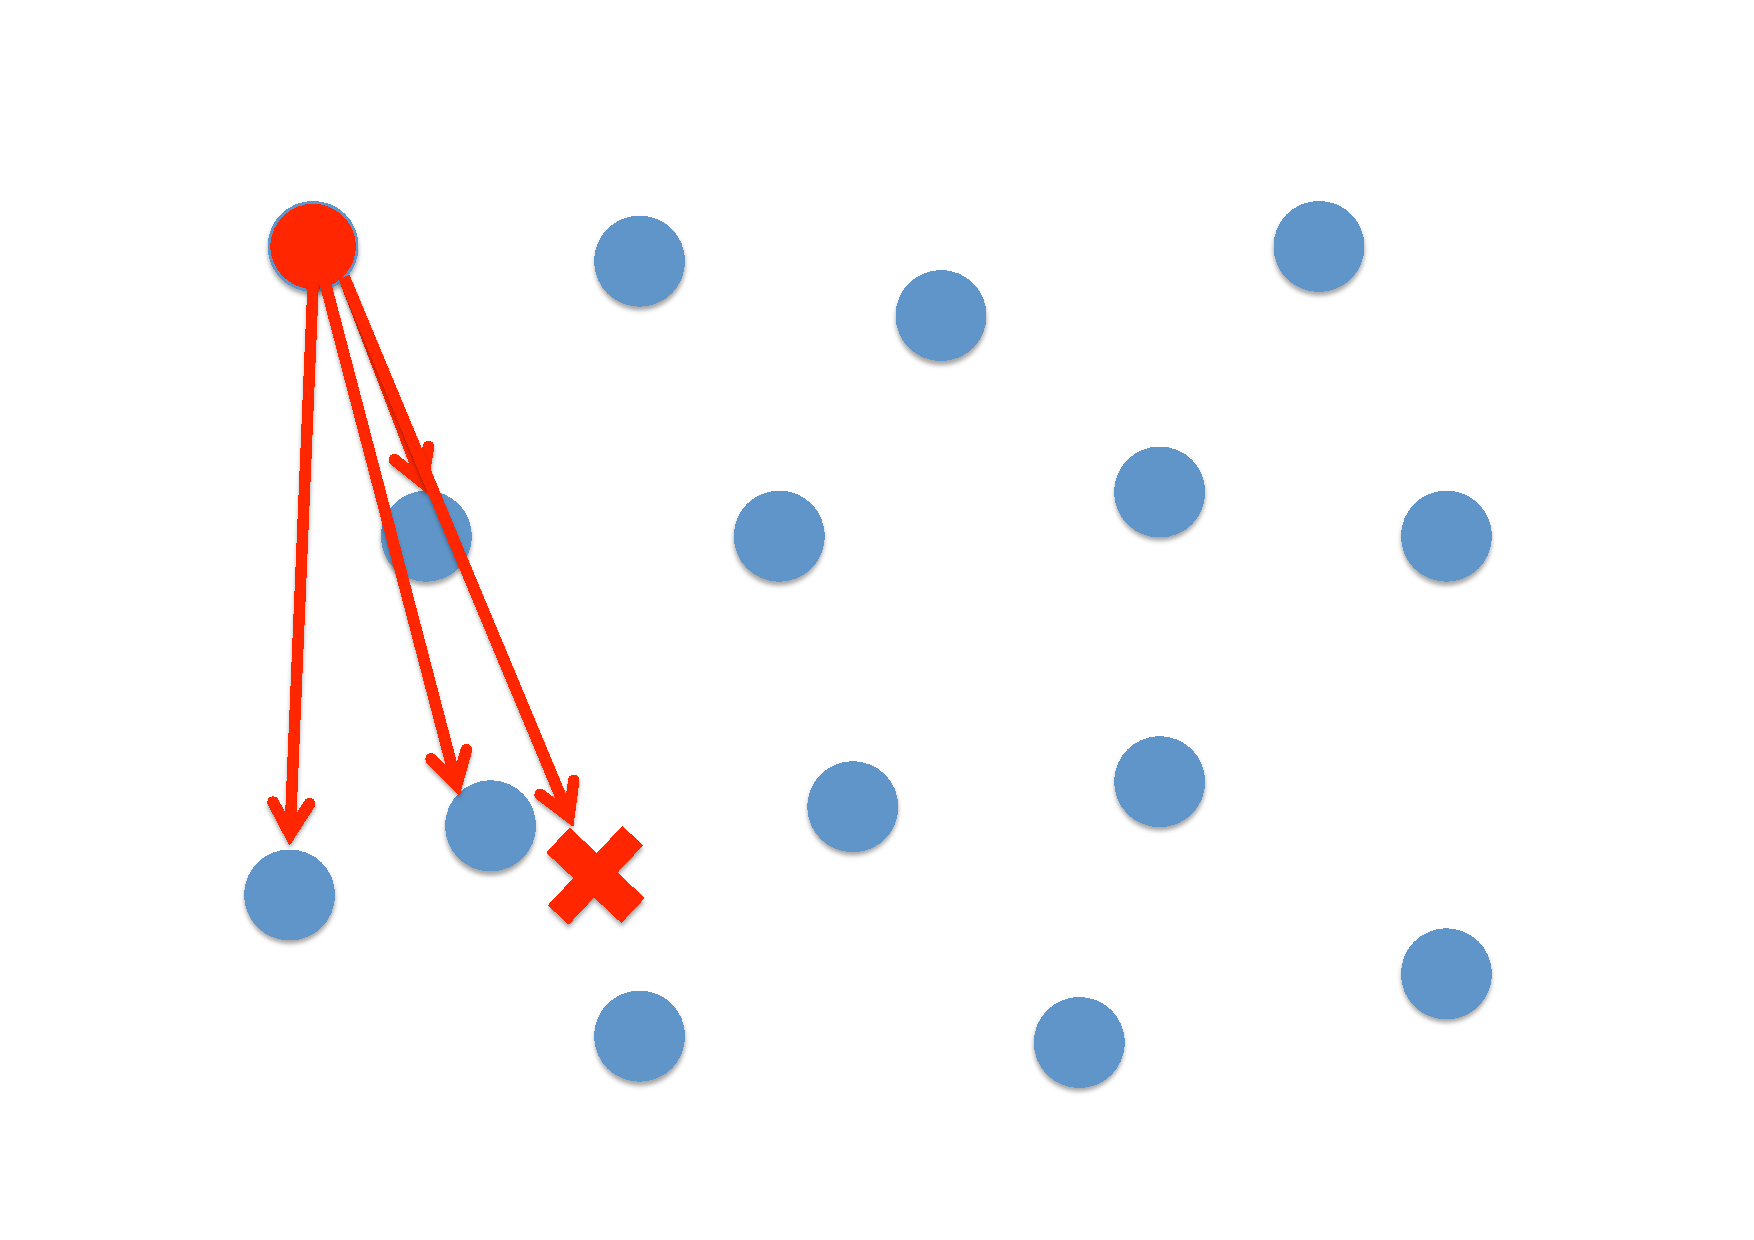
\includegraphics[width=1\textwidth]{pics/fault2}
  \end{center}
\end{figure}

}

\frame{
\frametitle{The Academic View: Data Dissemination}
\framesubtitle{Design Alternatives: One to All}

\begin{figure}[h]
  \begin{center}
  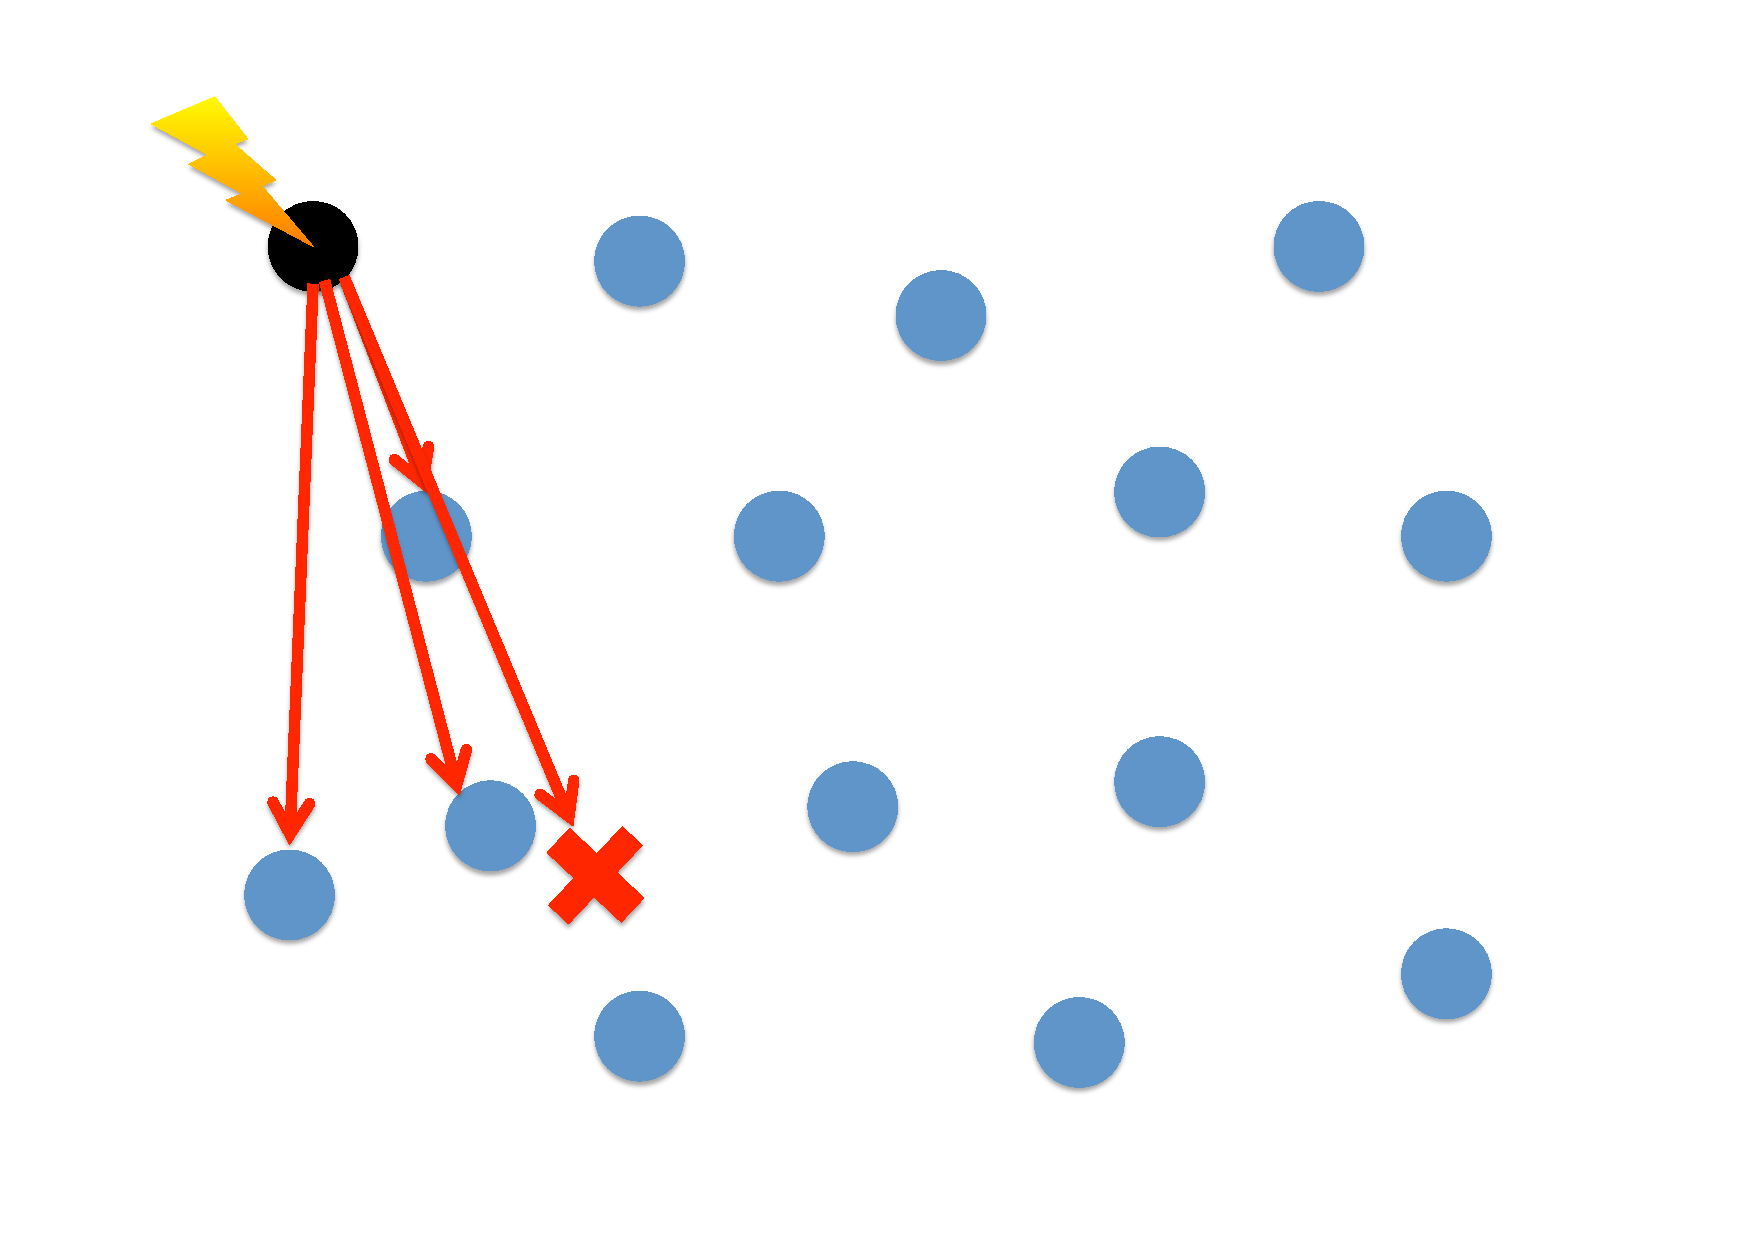
\includegraphics[width=1\textwidth]{pics/fault3}
  \end{center}
\end{figure}

}

\subsection{Design Alternatives: Spanning Tree}

\frame{
\frametitle{The Academic View: Data Dissemination}
\framesubtitle{Design Alternatives: Spanning Tree}

}

\subsection{Design Alternatives: Flood}

\frame{	
\frametitle{The Academic View: Data Dissemination}
\framesubtitle{Design Alternatives: Flood}

}

\subsection{Design Alternatives: Gossip}

\frame{
\frametitle{The Academic View: Data Dissemination}
\framesubtitle{Design Alternatives: Gossip}

}

\subsection{Design Alternatives: Embedded Tree}

\frame{
\frametitle{The Academic View: Data Dissemination}
\framesubtitle{Design Alternatives: Embedded Tree}

}

\section{Embedded Tree: Plumtree Protocol}

\frame{
\frametitle{Embedded Trees: Plumtree Protocol}
\framesubtitle{Building the Tree}

}


\frame{
\frametitle{Embedded Trees: Plumtree Protocol}
\framesubtitle{Recovering the Tree}

}


\frame{
\frametitle{Embedded Trees: Plumtree Protocol}
\framesubtitle{Sharing the Tree}

}

\frame{
\frametitle{Embedded Trees: Plumtree Protocol}
\framesubtitle{Experimental Evaluation}

}



\section{The Industry View: Cluster Metadata Management}

\frame
{
	\frametitle{Outline}
{
\small
	\tableofcontents[currentsection,hideallsubsections]
}
}

\subsection{Global Information, Needed Locally}
\frame{
\frametitle{The Industry View: Cluster Metadata Management}
\framesubtitle{Global Information, Needed Locally}
\begin{block}{Operational Information}
  Mebership, Ownership, Transfers, Capabilities
\end{block}

\begin{block}{Configuration}
  Replica Counts, Backends, Is Feature X Enabled?
\end{block}

\begin{block}{Monitoring Data}
  Transfer Statistics, Background Work Tracking, Self-Monitoring
\end{block}
}

\subsection{Requirements}
\frame{
\frametitle{The Industry View: Cluster Metadata Management}
\framesubtitle{Requirements}
\begin{itemize}
  \item Failure Tolerance
  \begin{itemize}
    \item Disable malicious clients despite network partitions
    \item Add new nodes despite others being down
  \end{itemize}
  \pause
  \item Quick Convergence
  \begin{itemize}
    \item Become aware of new nodes ASAP
    \item Keep monitoring data as fresh as possible
  \end{itemize}
  \pause
  \item Minimal Resource Usage
  \begin{itemize}
    \item Goal is to speed up, not slow down, foreground work
    \item Network is needed for the data!
  \end{itemize}
  \pause
  \item AP typically, CP rarely necessary
\end{itemize}
}

%To Jordan: Add your sub sections / main slides here
\section{Cluster Metadata Management In Riak}

\frame
{
	\frametitle{Outline}
{
\small
	\tableofcontents[currentsection,hideallsubsections]
}
}

%To Jordan: Add your sub sections / main slides here

\subsection{Implementations}
\frame{
\frametitle{Cluster Metadata Management In Riak}
\framesubtitle{Implementations}
\begin{block}{0.x}
\begin{itemize}
  \item Peer Service: Classic Anti-Entropy Protocol
  \item Data Dissemination: Same
\end{itemize}
\end{block}
\begin{block}{1.x}
\begin{itemize}
  \item Peer Service: Static Graph Overlay w/ Anti-Entropy
  \item Data Dissemination: Same
\end{itemize}
\end{block}
\begin{block}{2.x}
\begin{itemize}
  \item Peer Service: Static Graph Overlay w/ Anti-Entropy
  \item Data Dissemination: Sender-Based Embedded Trees
\end{itemize}
\end{block}
}

\subsection{Motivations}
\frame{
\frametitle{Cluster Metadata Management In Riak}
\framesubtitle{Motivations}
\begin{block}{0.x to 1.0}
\begin{itemize}
  \item Anti-Entropy is Reliable but Slow to Converge
  \item Improve Convergence Time, Specifically in Failure Scenarios
\end{itemize}
\end{block}
\begin{block}{1.x to 2.0}
\begin{itemize}
  \item Static Graph Overlay/Anti-Entropy have several issues:
    \begin{itemize}
      \item Too Much Network Overhead
      \item Improved Convergence Only Needed for Subset of Data
      \item Cold Rumor Mongering
    \end{itemize}
  \item Improve Resource Usage and Stability
\end{itemize}
\end{block}
}

\subsection{Plumtree: From Academia to Industry}
\frame{
\frametitle{Cluster Metadata Management In Riak}
\framesubtitle{Plumtree: From Academia to Industry}
\begin{block}{Connectivity}
``all nodes should have in their partial views...another correct node'' is not an invariant we can maintain
\end{block}
\begin{block}{System Model}
Must consider dropped, delayed, duplicated* messages in addition to node failures
\end{block}
\begin{block}{Topology}
Peer Service is Fully Connected (as is Erlang)
\end{block}
\begin{block}{Membership}
Operator-controlled instead of reactive (failure detector is implemented separately from peer service)
\end{block}
}

\subsection{Extending Plumtree}
\frame{
\frametitle{Cluster Metadata Management In Riak}
\framesubtitle{Extending Plumtree}
\begin{block}{What happens if Lazy Messages are Dropped?}
Add to Outstanding Set. Remove on Graft or Ack
\end{block}
\begin{block}{Handling Extreme Failures}
Back protocol by random anti-entropy with peers that are not in eager or lazy sets
\end{block}
\begin{block}{Shared vs. Sender-Based Trees}
Sender-Based. Minimize overhead w/ Lazy Construction
\end{block}
}

\subsection{Measurements}
\frame{
\frametitle{Cluster Metadata Management In Riak}
\framesubtitle{Measurements}
\begin{itemize}
\item Reduced convergence time (measured in LDH) by 66\%
\item Reduced needless message overhead in stable state 99.9\%
\item \% Failures before needing to rely on anti-entropy good for small clusters (near 90\%) but decreased quickly for larger clusters (under 50\%)
\end{itemize}
}

\subsection{Peer Service Tuning}
\frame{
\frametitle{Cluster Metadata Management In Riak}
\framesubtitle{Peer Service Tuning}
\begin{itemize}
\item Want to increase percent failures we can tolerate before relying on anti-entropy
\item Fanout of tree given to us by peer service matters
\item For clusters > 10 nodes, fanout = ln(cluster size) + 1
\item With our use of multiple trees, more peer service tuning may be necessary
\end{itemize}
}


\section{The Academic View: When One Tree is not Enough}

\frame
{
	\frametitle{Outline}
{
\small
	\tableofcontents[currentsection,hideallsubsections]
}
}

\subsection{Understanding The Problem}

\frame{
\frametitle{The Academic View: When One Tree is not Enough}
\framesubtitle{Understanding The Problem}

}

\subsection{Naive Solutions}

\frame{
\frametitle{The Academic View: When One Tree is not Enough}
\framesubtitle{Naive Solutions}

}


\subsection{Other Solutions}

\frame{
\frametitle{The Academic View: When One Tree is not Enough}
\framesubtitle{Other Solutions}

}

\subsection{Understanding The Goal}

\frame{
\frametitle{The Academic View: When One Tree is not Enough}
\framesubtitle{Understanding The Goal}

}


\section{The Thicket Protocol}

\frame
{
	\frametitle{Outline}
{
\small
	\tableofcontents[currentsection,hideallsubsections]
}
}

\subsection{Deploying the Trees}

\frame{
\frametitle{The Thicket Protocol}
\framesubtitle{Deploying the Trees}

}

\subsection{Recovering Trees}

\frame{
\frametitle{The Thicket Protocol}
\framesubtitle{Recovering Trees}

}

\subsection{Experimental Results}

\frame{
\frametitle{The Thicket Protocol}
\framesubtitle{Experimental Results}

}

\section{The Industry View: Improving Cluster Metadata Management}

%To Jordan: Add your sub sections / main slides here

\frame
{
	\frametitle{Outline}
{
\small
	\tableofcontents[currentsection,hideallsubsections]
}
}

\subsection{Measuring Interior Nodes}
\frame{
\frametitle{The Industry View: Improving Cluster Metadata Management}
\framesubtitle{Measuring Interior Nodes}
\begin{block}{10 Nodes}
  \begin{itemize}
    \item 4 of 10 nodes are interior in 3 of 10 trees
    \item 3 of 10 nodes are interior in 4 of 10 trees
    \item 3 of 10 nodes are interior in 5 of 10 trees
  \end{itemize}
\end{block}
\begin{block}{20 Nodes}
  \begin{itemize}
    \item 4 nodes are interior only when roots
    \item 16 nodes are interior in 5 or more trees
  \end{itemize}
\end{block}
\begin{block}{80 Nodes}
  \begin{itemize}
    \item 4 nodes are interior only when roots
    \item 36 of 80 nodes are interior in > 25\% of trees
  \end{itemize}
\end{block}
}

\subsection{The Peer Service's Role}
\frame{
\frametitle{The Industry View: Improving Cluster Metadata Management}
\framesubtitle{Improving Interior Node Counts}
\begin{itemize}
\item Coupling between fanout, number of trees, and how many times a node must be interior
\item Height of initial trees constructed by peer service
\end{itemize}
}


\section{The Future of Cluster Metadata in Riak}

%To Jordan: Add your sub sections / main slides here

\frame
{
	\frametitle{Outline}
{
\small
	\tableofcontents[currentsection,hideallsubsections]
}
}


\subsection{Expand Usage}
\frame{
\frametitle{The Future of Cluster Metadata in Riak}
\framesubtitle{Expand Usage}
\begin{block}{Exploring Thicket}
\begin{itemize}
  \item Research Area
\end{itemize}
\end{block}
\begin{block}{Migration \& New Data}
\begin{itemize}
  \item Move data from 1.x subsystem to 2.x subsystem
  \item Store data we couldn't before
\end{itemize}
\end{block}
\begin{block}{WAN Replication}
\begin{itemize}
  \item Integrate with Riak's Multi-Site Replication
  \item Abstract Messaging Layer
\end{itemize}
\end{block}
}

\section{Summary}

\frame
{
	\frametitle{Outline}
{
\small
	\tableofcontents[currentsection,hideallsubsections]
}
}

\frame{
\frametitle{Summary}
\framesubtitle{}

}

\frame
{
	\frametitle{}
	\framesubtitle{}

	\begin{center}
		{\Huge
			Thanks.
		}
	\end{center}
}

\end{document}
